%%%%%%%%%%%%%%%%%%%%%%%%%%%%%%%%%%%%%%%%%
% a0poster Portrait Poster
% LaTeX Template
% Version 1.0 (22/06/13)
%
% The a0poster class was created by:
% Gerlinde Kettl and Matthias Weiser (tex@kettl.de)
% 
% This template has been downloaded from:
% http://www.LaTeXTemplates.com
%
% License:
% CC BY-NC-SA 3.0 (http://creativecommons.org/licenses/by-nc-sa/3.0/)
%
%%%%%%%%%%%%%%%%%%%%%%%%%%%%%%%%%%%%%%%%%

%----------------------------------------------------------------------------------------
%	PACKAGES AND OTHER DOCUMENT CONFIGURATIONS
%----------------------------------------------------------------------------------------

\documentclass[a0,portrait]{a0poster}

\usepackage{subcaption} 
\usepackage{natbib} % use citep
\usepackage{ wasysym } % astrosun symbol.
\usepackage{gensymb} % degree symbol
\usepackage{multicol} % This is so we can have multiple columns of text side-by-side
\columnsep=100pt % This is the amount of white space between the columns in the poster
\columnseprule=3pt % This is the thickness of the black line between the columns in the poster

\usepackage[svgnames]{xcolor} % Specify colors by their 'svgnames', for a full list of all colors available see here: http://www.latextemplates.com/svgnames-colors

%\usepackage{times} % Use the times font
\usepackage{palatino} % Uncomment to use the Palatino font

\usepackage{graphicx} % Required for including images
\graphicspath{{figures/}} % Location of the graphics files
%\usepackage{booktabs} % Top and bottom rules for table
\usepackage[font=small,labelfont=bf]{caption} % Required for specifying captions to tables and figures
%\usepackage{amsfonts, amsmath, amsthm, amssymb} % For math fonts, symbols and environments
\usepackage{wrapfig} % Allows wrapping text around tables and figures
\usepackage{url}

%\usepackage{realboxes}

\renewcommand{\emph}[1]{\textbf{\color{blue}#1}}

\newcommand{\vs}[1] {\textbf{\textcolor{red}{#1}}}

\newcommand{\ECM}[1] {\textbf{\textcolor{magenta}{#1}}}

%\renewcommand{\section}[2]{\Colorbox{lightgray}{\noindent {\Large \textbf{#2}} \hfill}}

%\usepackage{lipsum}

\begin{document}

%----------------------------------------------------------------------------------------
%	POSTER HEADER 
%----------------------------------------------------------------------------------------

% The header is divided into two boxes:
% The first is 75% wide and houses the title, subtitle, names, university/organization and contact information
% The second is 25% wide and houses a logo for your university/organization or a photo of you
% The widths of these boxes can be easily edited to accommodate your content as you see fit

\begin{minipage}[b]{0.75\linewidth}
  \Huge \textbf{ 	Prospects about X- and gamma-ray counterparts of gravitational wave signals with INTEGRAL}\\[1cm] % Title
  \large \textbf{P.~Bacon, V.~Savchenko and E.~Chassande-Mottin \vs{we should think to add INTEGRAL collaboration}}\\[1cm] % Author(s)
  \normalsize APC, Univ Paris Diderot, CNRS/IN2P3, CEA/Irfu, Obs. de Paris, Sorbonne Paris Cit\'e, France\\
  \large \texttt{philippe.bacon@apc.in2p3.fr}\\
\end{minipage}
%
\begin{minipage}[b]{0.25\linewidth}
	
\includegraphics[scale=.8]{logo.png}
\end{minipage}

\vspace{1cm} % A bit of extra whitespace between the header and poster content

%----------------------------------------------------------------------------------------

\begin{multicols}{2} % This is how many columns your poster will be broken into, a portrait poster is generally split into 2 columns


 \begin{abstract}
   By extrapolating the number of detections made during the first
   LIGO science run, tenths of gravitational wave signals from binary
   black hole mergers are anticipated in upcoming LIGO Virgo science
   runs. Finding an electromagnetic counterpart to compact binary
   merger events would be a landmark discovery. The search for such
   counterpart is challenging for a number of reasons, such as the
   poor resolution of source position reconstruction from the
   gravitational wave observations alone, and the weakness of the
   expected electromagnetic signal. In this poster, we evaluate the
   ability of current wide-field X- and gamma-ray telescopes aboard
   INTEGRAL to find such counterparts. We present the result of an
   end-to-end simulation for estimating the fraction of the sources
   that can be followed up, and the fraction of counterparts that can
   be detected based on different models.
 \end{abstract}

 % satellite : What fraction of GW events can be recovered in the EM spectrum ?
 % What should be the statistical significance of the GW and the EM events to
 % claim a confident joint detection ? \textcolor{blue}{BOTTOM LINE RESULTS : We
 % show that...}

\section*{Motivations}

On Sep 14 2015, the two LIGO interferometers made the first direct detection of
gravitational waves (GW). A next step would be to detect an electromagnetic (EM)
counterpart associated to a GW event. This would inaugurate a new,
multimessenger era in the astronomy history. We address the question of the
joint detectability of GW events by Advanced Virgo and Advanced LIGO, and
associated EM events at high-energies by the INTEGRAL mission. We produce an
\emph{end-to-end simulation of the search for gravitational-waves from binary
  neutron star mergers \textit{and} follow-up observation seeking a possible
  electromagnetic counterpart at high-energies.} This study is similar to the
one done in \cite{2016arXiv160606124P} with Fermi.

\section*{Monte-Carlo simulation of gravitational-wave events from neutron-star binary mergers}

We start with a simulated catalogue of 6 millions Milky Way-like galaxies
distributed to $z\sim 0.12$. To those galaxies, we associate binary neutron star
(BNS) mergers with mass distribution and rate of R=$23.5 M\mathrm{yr}^-3$ per galaxy
according to Model A ($Z_{\astrosun}$ metallicity) of
\cite{dominik12:_doubl_compac_objec}. This results in a population of 14\,000
mergers for a $100$ year simulation.

\begin{center}\vspace{.5cm}
    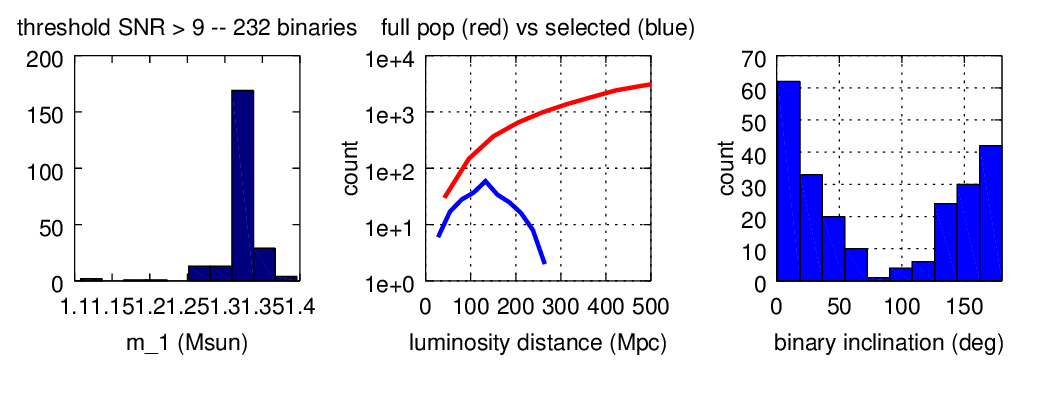
\includegraphics[width=30cm]{figures/summary_plot.png}
\end{center}

We simulate GW signals corresponding to the binary mergers (using model
``TaylorT4'') and inject them into Gaussian noise coloured according to the
``optimistic'' power-spectral density anticipated for the 2nd LIGO/Virgo run O2
\cite{lrr-2016-1}. We select signals with $\mathrm{SNR}_{\mathrm{combined}} > 9$
corresponding to a false-alarm rate $\mathrm{FAR} < 1/\mathrm{month}$. The average range
BNS is 126 Mpc for this selection.

The resulting 232 binaries are distributed randomly in time during the expected
period of O2 from Nov 2016 to May 2017 (6 months). We recover GW signals using
matched-filtering techniques and reconstruct the posterior skymaps giving the
position of the source with the BAYESTAR pipeline \cite{PhysRevD.93.024013}.

% SNR threshold HL = 6 : RHO_thres_NETWORK = sqrt(rho_H**2 + rho_L**2) = 6
% On one hand, the signal only takes the inspiral phase into account via the use of non-spinning waveform 'TaylorF4ThreePN'.
% As we want to reproduce an analogue study with \textsc{INTEGRAL} it justifies why our simulation settings are aligned on their work. This will allow further comparisons.
% As a transition towards the details of the EM emission we estimated the total GW emitted energy $E_{\mathrm{EM}}$ of the simulated BNS systems thanks to Bernuzzi et al. \cite{2016PhRvD..94b4023B}, ie.  $E_{GW} \sim 1.5 \% \, M c^{2}$ where M is the total mass of the binary.

\section*{Electromagnetic emission model from neutron-star binary mergers}

Compact binary mergers involving at least one neutron star are considered to be
plausible progenitors of short gamma-ray bursts (GRB). Short GRBs constitute a
subset of the whole GRB population with typical duration shorter than $\sim$2
seconds. Short GRBs have also a harder spectrum.  Prompt emission is attributed
to dissipation within the collimated ultra-relativistic jet and is therefore
strongly beamed. It is followed by slowly decaying afterglow, observed from
radio to GeV, produced by the interaction between the ejecta and the ambient
medium surrounding the GRB progenitor. Afterglow emission is originally also
strongly beamed, but as the outflow decelerates, the emission becomes
progressively more isotropic.

\emph{In our simulation we assume that every BNS merger is associated with a short
gamma-ray burst. We simulate synthetic prompt GRB and a hard X-ray afterglow,
assuming the following simplified model.}

\subsection*{Prompt emission}
We model the prompt emission spectrum by a broken power-law, so-called the Band
\cite{band93} model. For simplicity we assume the same prompt emission spectrum
for all synthetic GRB, with $\alpha_{\mathrm{BAND}} = - 0.5$ and
$E_{\mathrm{peak}} = 600$ \, keV, close to the average short GRB spectrum
observed by Fermi/GBM \cite{gruber14}.  \ECM{Not clear: In the case of short
  GRBs, the slope above the peak energy is not well constrained, and the
  spectrum can be well described by a cutoff power-law. -- Would this be
  correct?: Above the peak energy, the spectrum can be well described by a
  cut-off power-law, although the slope is not well constrained.} We also assume
fixed duration of the prompt emission of 1 second and fixed isotropic equivalent
luminosity of $10^{50}~$erg~cm$^{-2}$~s$^{-1}$.

The principal source of uncertainty on rate of GRB detections associated with
the BNS mergers is the beaming factor of the prompt emission. We assume a fixed
beaming angle of 10 degrees. This angle is roughly compatible with the
observations of the total short GRB rate inferred from our BNS population.

\subsection*{Hard X-ray afterglows}

We assume that every BNS merger produces a hard X-ray afterglow. Although
afterglows in the hard X-rays are rarely observed, it is not unreasonable to
assume that they are as frequent as gamma-rays, but observed much less
frequently due to observational limitations.

There are indications that such afterglows are present in the most luminous GRBs
occuring about once in few months (2\% of the sky observed by INTEGRAL).  When
hard X-ray afterglows are observed, INTEGRAL observations reveals very high
SNR. For instance, GRB120711A was seen in INTEGRAL/ISGRI and JEM-X for about 8
hours \cite{martincarillo14}. The bright hard X-ray emission afterglow found to
be related to the bright gamma-ray afterglow, observed by Fermi/LAT in the
energy range above 100 MeV. In particular, it had the same spectrum, powerlaw
with a slope of -2.

We assume a spectrum similar to GRB120711A, but rescaled to the total EM
luminosity of a typical short GRB - $10^{50}~$erg$^{-2}~$s$^{-1}$. In most of
the cases the outflow is not aligned with the line of sight. To compute the
afterglow light curve as seen off-axis, we assume that the emission is
originating in a single small relativistically moving region, decelerating from
initial $\Gamma_0$=200 over a deceleration time scale 100~s (see Model~I in
\cite{xxx}).

% Power law model see Eq(1) of 'THE FERMI GBM GAMMA-RAY BURST SPECTRAL CATALOG: FOUR YEARS OF DATA' - Gruber et al 

\begin{center}
    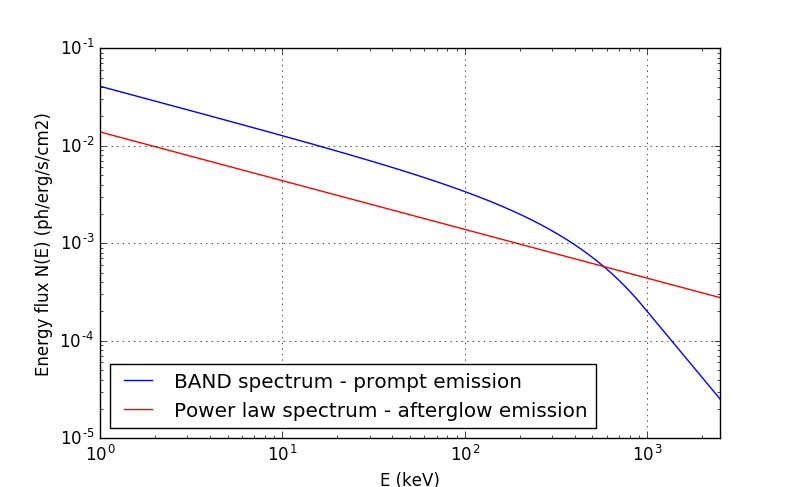
\includegraphics[height=10cm]{figures/spectra.png}
    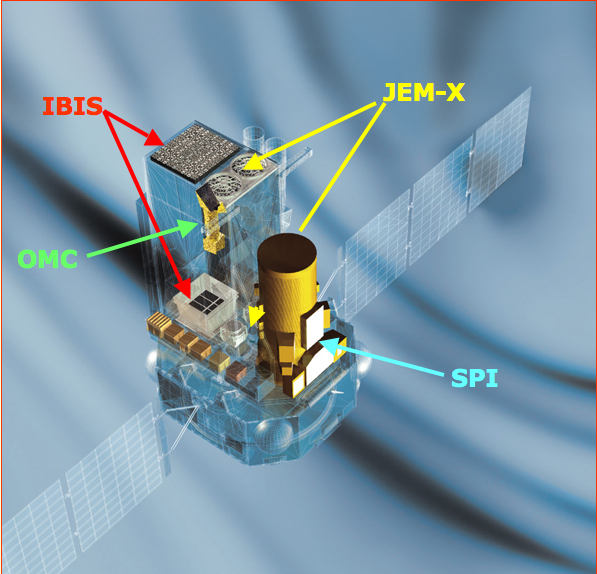
\includegraphics[height=10cm]{figures/INTEGRAL.jpg}
    \captionof{figure}{(\textit{Left}) Prompt and afterglow emission spectra from SGRBs systems. Fluxes have been normalized with respect to the INTEGRAL finite energy band $\left[ 75 \, , 2000 \right] \, \mathrm{keV}$. (\textit{Right}) Instruments embarked on INTEGRAL satellite.}
    \label{spectra}
\end{center}

\section*{The INTEGRAL mission and possible follow-up strategies}

%\ECM{Describe the relevant instruments here. Energy range covered. FOV.}
% LINK : http://www.cosmos.esa.int/web/integral/instruments-ibis
%        http://www.cosmos.esa.int/web/integral/instruments-spi

The INTEGRAL satellite carries a combination of pointing instruments, covering
wide energy range from 3 keV to 10 MeV (ISGRI, PICsIT, JEM-X, and SPI) with
field of view up to 900 deg$^2$. \emph{Active follow-up:} We assume that every
GW alerts reported by LIGO/Virgo is followed by INTEGRAL pointings. Typical
latency of INTEGRAL observation is about 1 day but may be lower in some
circumstances. We compute the flux at several moments of time, and compare it
with ISGRI sensitivity in 100~ks observation. \emph{Passive follow-up:} In
addition, INTEGRAL/SPI-ACS and IBIS are capable of detecting bright transients
from every sky direction.

% As GRBs will then be monitored thanks to the SPI-ACS and IBIS instruments embarked on the \textsc{INTEGRAL} satellite mission, we thus have to convert the energy information into some constraints acting on the detectable energy flux by those instruments. The emitted EM flux is hence truncated to the \textsc{INTEGRAL} finite energy band $\left[ 75 \, , 2000 \right] \, \mathrm{keV}$. \\

\section*{Results}

\subsection*{Prompt -- Passive follow-up}

\begin{center}
    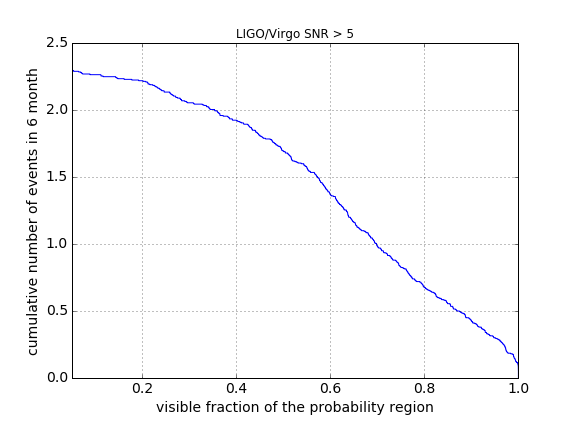
\includegraphics[height=8cm]{figures/covered_region.png}
    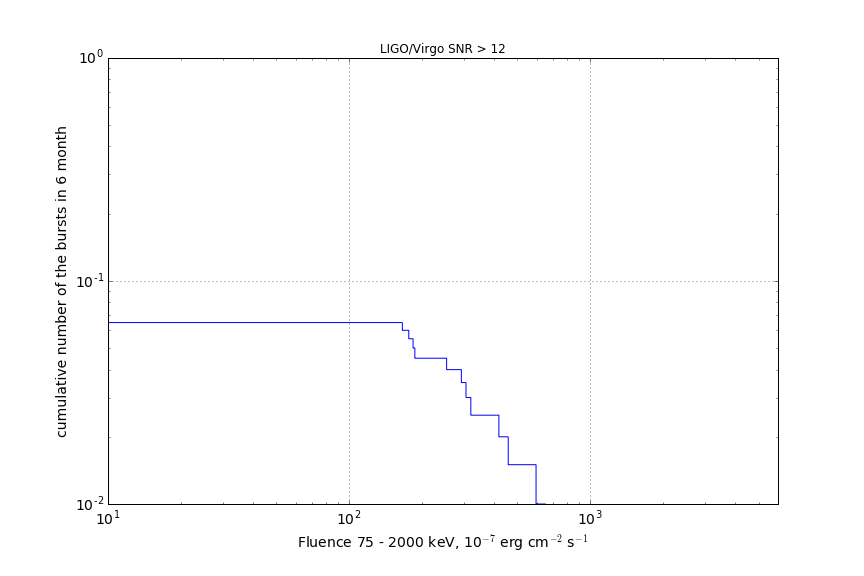
\includegraphics[height=8cm]{figures/fluence_distribution_12.png}
    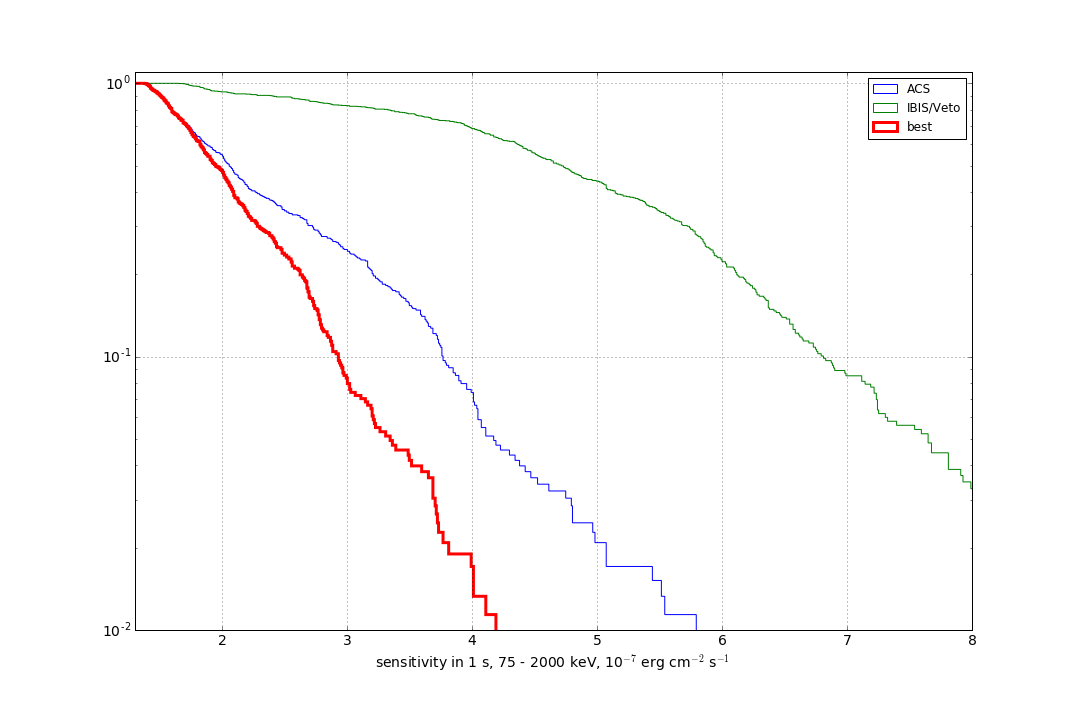
\includegraphics[height=8cm]{figures/sensitivity_distribution_pe.png}
    \captionof{figure}{(\textit{Left}) Cumulative distribution of the fraction of the LIGO/Virgo localization region accessible to INTEGRAL pointed follow-up observation in the LIGO/Virgo O2 run. (\textit{Middle}) Cumulative distribution of the detected fluences by INTEGRAL in the LIGO/Virgo O2 run.(\textit{Right}) Cumulative distribution of the sensitivity of the IBIS and SPI-ACS instruments.}
    \label{covered_region}
\end{center}

Choosing an isotropic sky distribution of our GW events, we show that
in every case where the Earth is within the GRB emission cone,
INTEGRAL detects prompt emission with significance at least 50~sigma.
The rate of detection is 0.5 in 6 month of O2 in the case of faint
LIGO events (\vs{SNR}) and 0.1 in 6 month in the case of loud events
(\vs{SNR}).

\subsection*{Afterglow -- Instrument repointing}

Due to observational constrains, only a fraction of the GW localization
region can be observed by INTEGRAL. For each event we compute the
total localization probability within the observable region, and find
that in \vs{1\%} of the cases 99.7\% of the localization can be
observed. However, if the complete available region will be followed-up
every time, in total 80\% of the true source locations will be
covered.

We find that the expected rate of 5~sigma detections is only about
\vs{0.01} events in 6 month of O2. We explore also another
possibility, that 10\% of the events launch much more energetic
outflow, in agreement with luminosities observed in real short
GRBs. In this case we expect about 0.1 events seen in 6 month. 

We stress that the afterglow prediction is particularly sensitive to
on assumptions on rather uncertain source model, and we assume only
one, yet realistic, option.

\begin{center}\vspace{.5cm}
  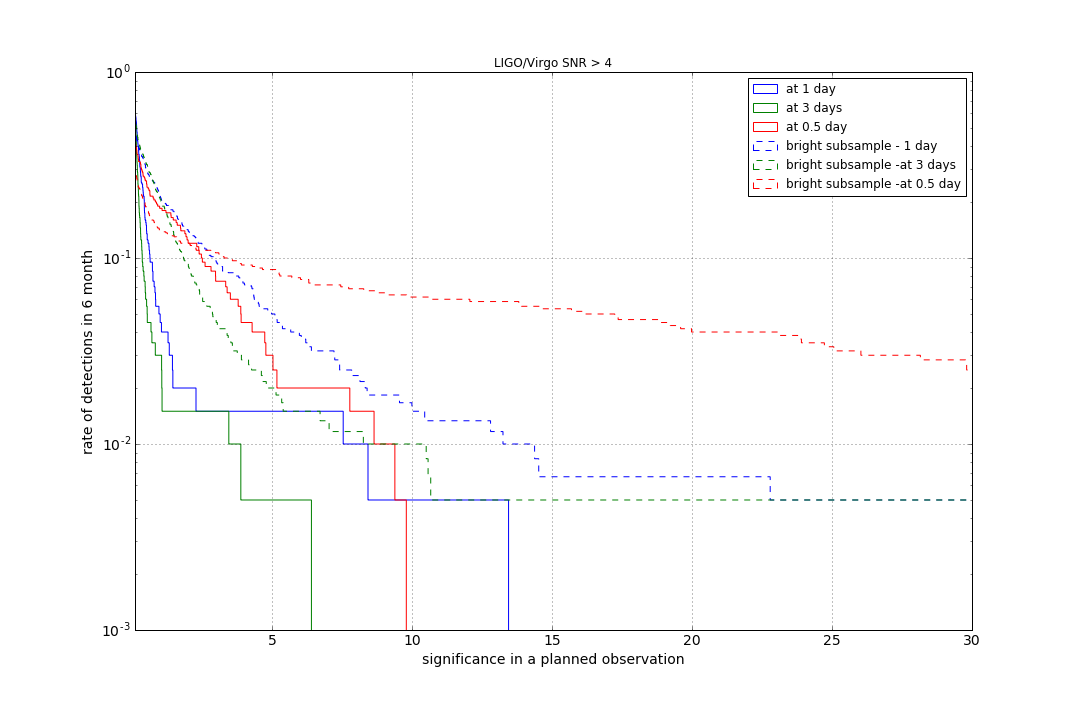
\includegraphics[width=10cm]{figures/significance_vs_rate_af.png}
  \captionof{figure}{Significance distribution on detected sources
    depending on time delay after the prompt emission.}
    \label{covered_region}
\end{center}

The left figure brings an answer to the second question : what is the duration
limit after the prompt emission within which we are able to detect the SGRB
source ?

% \section*{Conclusions}

% Among compact objects populations GRBs are the most promising astrophysical
% sources from which we can expect a gamma-ray emission loud enough to be
% associated to GW radiation sources and thus be detectable with adequate
% instruments. We show in this poster that INTEGRAL is the appropriate to ensure a
% follow-up for both the prompt and afterglow emissions, thanks to the IBIS and
% SPI-ACES instruments.


%----------------------------------------------------------------------------------------
%	ACKNOWLEDGEMENTS
%----------------------------------------------------------------------------------------

\vspace{10mm}
\noindent {\normalsize \textbf{Acknowledgements}}

{\footnotesize 
  This research was supported in part by the ASTERICS grant. The authors would like to thank Barbara Patricelli for sharing data and Philippe Laurent for fruitful discussions. }
  %We thank ASTERICS. Barbara Patricelli for sharing data, Philippe Laurent for discussions}

%----------------------------------------------------------------------------------------
%	REFERENCES
%----------------------------------------------------------------------------------------

%\nocite{*} % Print all references regardless of whether they were cited in the poster or not
\bibliographystyle{plain} % Plain referencing style
\bibliography{bib_other} % Use the example bibliography file sample.bib

%----------------------------------------------------------------------------------------

\end{multicols}
\end{document}
